%%%%%%%%%%%%%%%%%%%%%%%%%%%%%%%%%%%%%%%%%
% University/School Laboratory Report
% LaTeX Template
% Version 3.0 (4/2/13)
%
% This template has been downloaded from:
% http://www.LaTeXTemplates.com
%
% Original author:
% Linux and Unix Users Group at Virginia Tech Wiki 
% (https://vtluug.org/wiki/Example_LaTeX_chem_lab_report)
%
% License:
% CC BY-NC-SA 3.0 (http://creativecommons.org/licenses/by-nc-sa/3.0/)
%
%%%%%%%%%%%%%%%%%%%%%%%%%%%%%%%%%%%%%%%%%

%----------------------------------------------------------------------------------------
%	PACKAGES AND DOCUMENT CONFIGURATIONS
%----------------------------------------------------------------------------------------
\documentclass{article}
\usepackage{amsmath}
\usepackage{amsfonts}
\usepackage{amssymb}
\usepackage{siunitx} % Provides the \SI{}{} command for typesetting SI units
\usepackage{graphicx} % Required for the inclusion of images
\setlength\parindent{0pt} % Removes all indentation from paragraphs
\renewcommand{\labelenumi}{\alph{enumi}.} % Make numbering in the enumerate environment by letter rather than number (e.g. section 6)
\def\thesection{\Alph{section}} % make the secions be index by letters
\usepackage[section]{placeins} % make sure figures are placed in the correct section
\usepackage{pdfpages}
\usepackage[version=3]{mhchem} % chemistry typesetting
%\usepackage{times} % Uncomment to use the Times New Roman font

%----------------------------------------------------------------------------------------
%	DOCUMENT INFORMATION
%----------------------------------------------------------------------------------------
\title{Engine Design \\ Pyralis Engine \\ MIT Rocket Team} % Title
\author{Matt Vernacchia and Nicholas Voce} % Author name
\date{ \today } % Date for the report

%----------------------------------------------------------------------------------------
% THE BODY OF THE REPORT
%---------------------------------------------------------------------------------------

\begin{document}
\section{Propellant Selection}
We require propellants which:
\begin{enumerate}
\item Are storable at room temperature (non-cryogenic).
\item Are able to be liquefied at room temperature ($\SI{295}{\kelvin}$) so as to have compact sized tanks.
\item Have a high vapour pressure at room temperature so that the propellants will self-pressurize the combustion chamber. This enables us to avoid using a turbopump or inert gas system to pressurize the combustion chamber, greatly simplifying the engine design.
\item Are non-toxic or low-toxicity.
\item Are low-cost and readily available.
\end{enumerate}
Nitrous oxide \ce{N2O} is the oxidizer most widely used in hobby rocketry. \ce{N20} and hydrogen peroxide are the only widely used oxidizer which can be liquid at room temperature, and \ce{N2O} is the less toxic and more stable of the two. \ce{N20} also presents a vapour pressure of $\SI{5.29}{\mega\pascal}$ at $\SI{295}{\kelvin}$, which is a sufficient combustion chamber pressure. Thus \ce{N2O} will be our oxidizer.\\
\begin{figure}[h!]
\centering
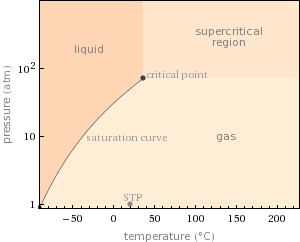
\includegraphics[width = 0.8\textwidth]{n2o_vap.png}
\caption{Vapour pressure curve of nitrous oxide} 
\label{n2o_vap}
\end{figure}
Alkane hydrocarbon fuels provide a high energy density and are comparatively cheap. All alkanes but methane (\ce{CH4}) can be liquefied at room temperature. Of these, ethane \ce{C2H6} presents the highest vapour pressure of $\SI{4.40}{\mega\pascal}$. Ethane has a similar vapour pressure curve and critical point to \ce{N2O}, making a convenient pairing. Therefore we will use ethane as our fuel.
\begin{figure}[h!]
\centering
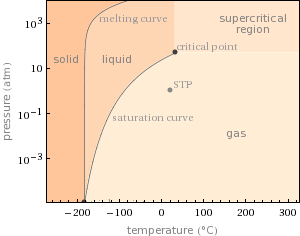
\includegraphics[width = 0.8\textwidth]{c2h6_vap.png}
\caption{Vapour pressure curve of ethane} 
\label{c2h6_vap}
\end{figure}
We will use a oxidizer to fuel ratio of $3:1$ by mass. This ratio is fuel-rich compared to the stoichiometric ratio. NASA's CEARUN tool predicts that this mixture will yield an adiabatic flame temperature of $\SI{1727}{K}$ \cite{CEARUN}. CEARUN tool also predicts that the fuel-rich burn will produce significant amounts of hydrogen ($0.41$ mole fraction), and carbon monoxide ( $0.27$ mole fraction). A oxidizer-rich burn would produce significant nitrogen and carbon dioxide by-products. As \ce{H2} and \ce{CO} are of lower molar mass than \ce{N2} and \ce{CO2}, a fuel-rich burn will produce lower exhaust molar mass and therefore higher specific impulse than an oxidizer-rich combustion process.
\section{Aerospike Nozzle}
Our engine will use an aerospike, an altitude-compensating nozzle featuring an annular expansion region with an inner solid boundary and an outer fluid boundary. As few aerospike nozzle engines have been produced (excepting the XRS-2200), creating and testing an aerospike engine would allow the team to make a real contribution to the cutting edge of aerospace engineering. A major difficulty with aerospike engines is cooling the spike. However at this small scale we can produce the spike from a material (i.e. graphite) which can survive prolonged exposure to the temperature of our exhaust gas without cooling. This eliminates the main factor which would make the use of an aerospike nozzle more difficult that the use of a De Laval nozzle.\\
\begin{figure}[h!]
\centering
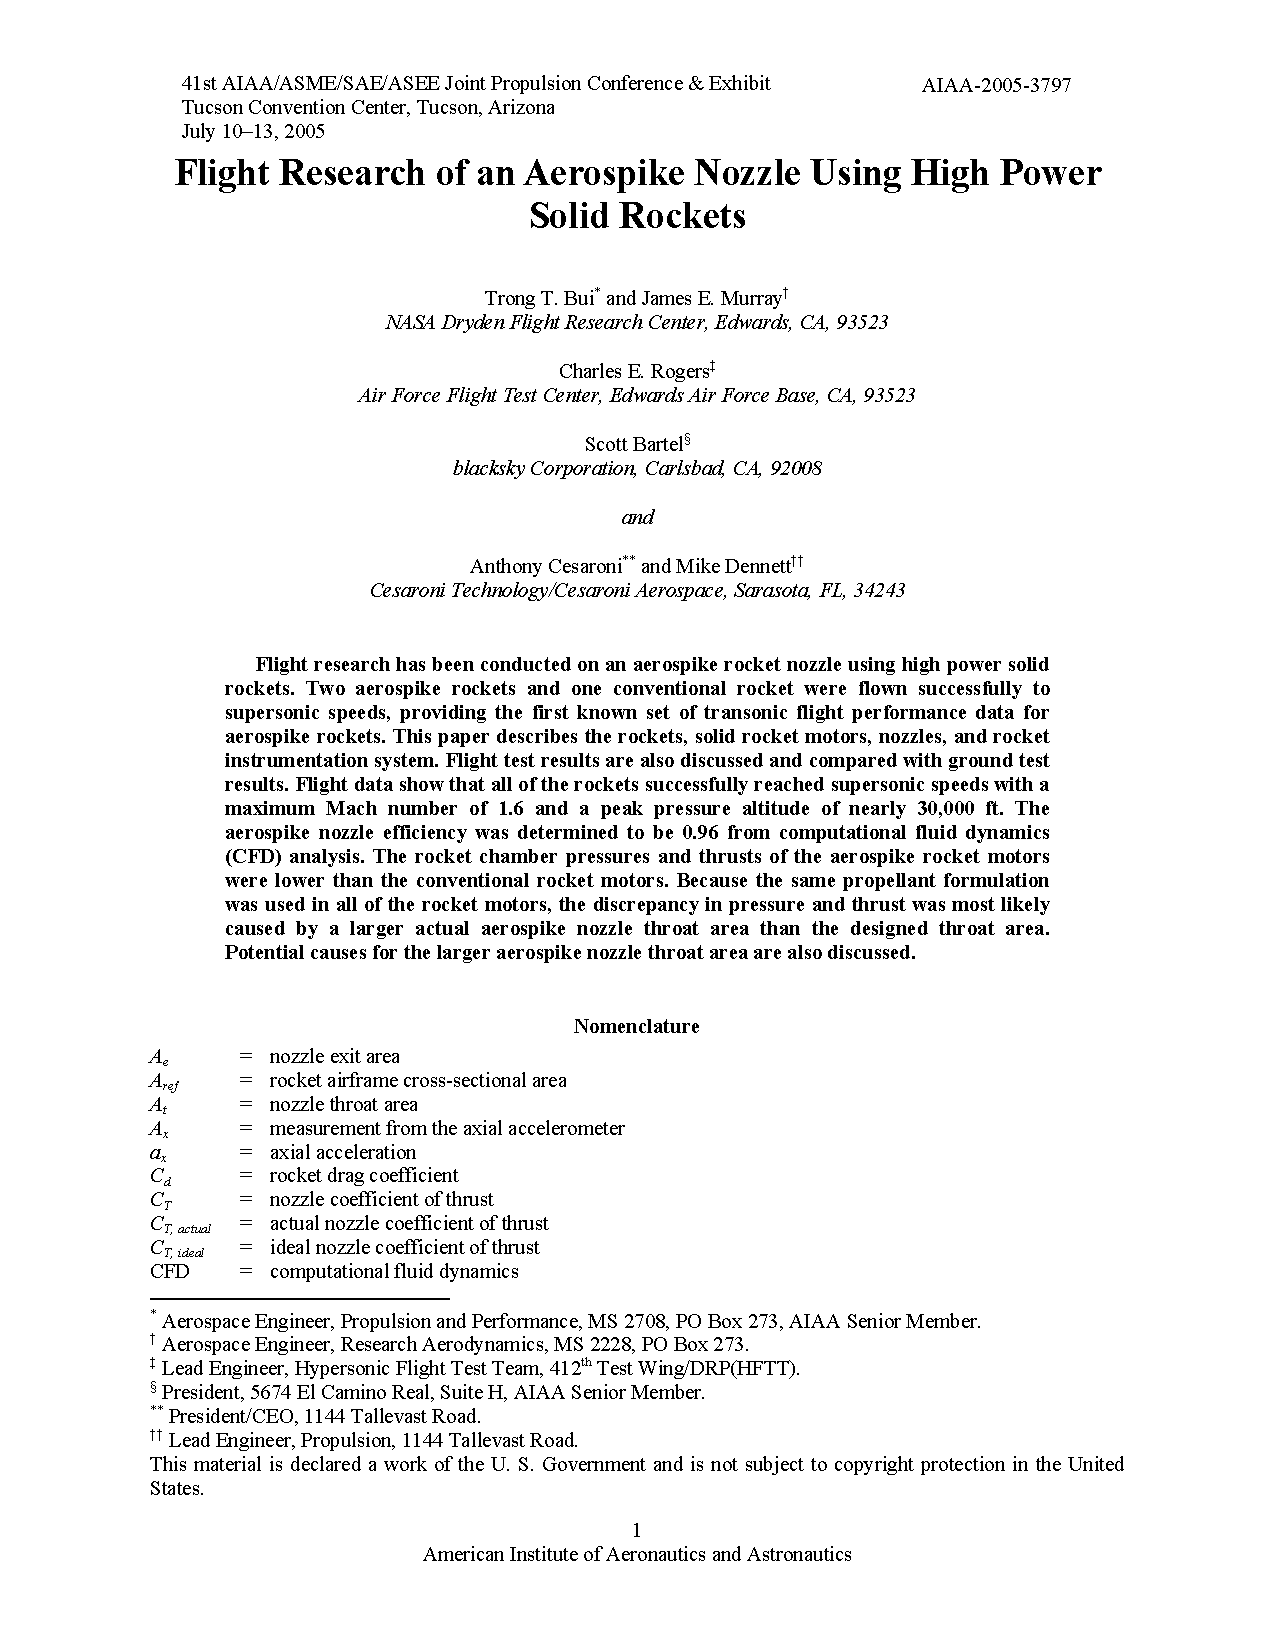
\includegraphics[width = 0.8\textwidth]{dryden_aerospike.png}
\caption{A small aerospike nozzle engine made by NASA Dryden} 
\label{dryden_aerospike}
\end{figure}
C.C. Lee presents a numerical algorithm for designing the contour of an aerospike nozzle and predicting the performance of the associated engine. Using his algorithm, we predict a thrust of approximately $\SI{700}{\newton}$ and a specific impulse of $\SI{390}{sec}$ for a $\SI{30}{\milli\metre}$ diameter nozzle (Fig \ref{spike_contour}).
\begin{figure}[h!]
\centering
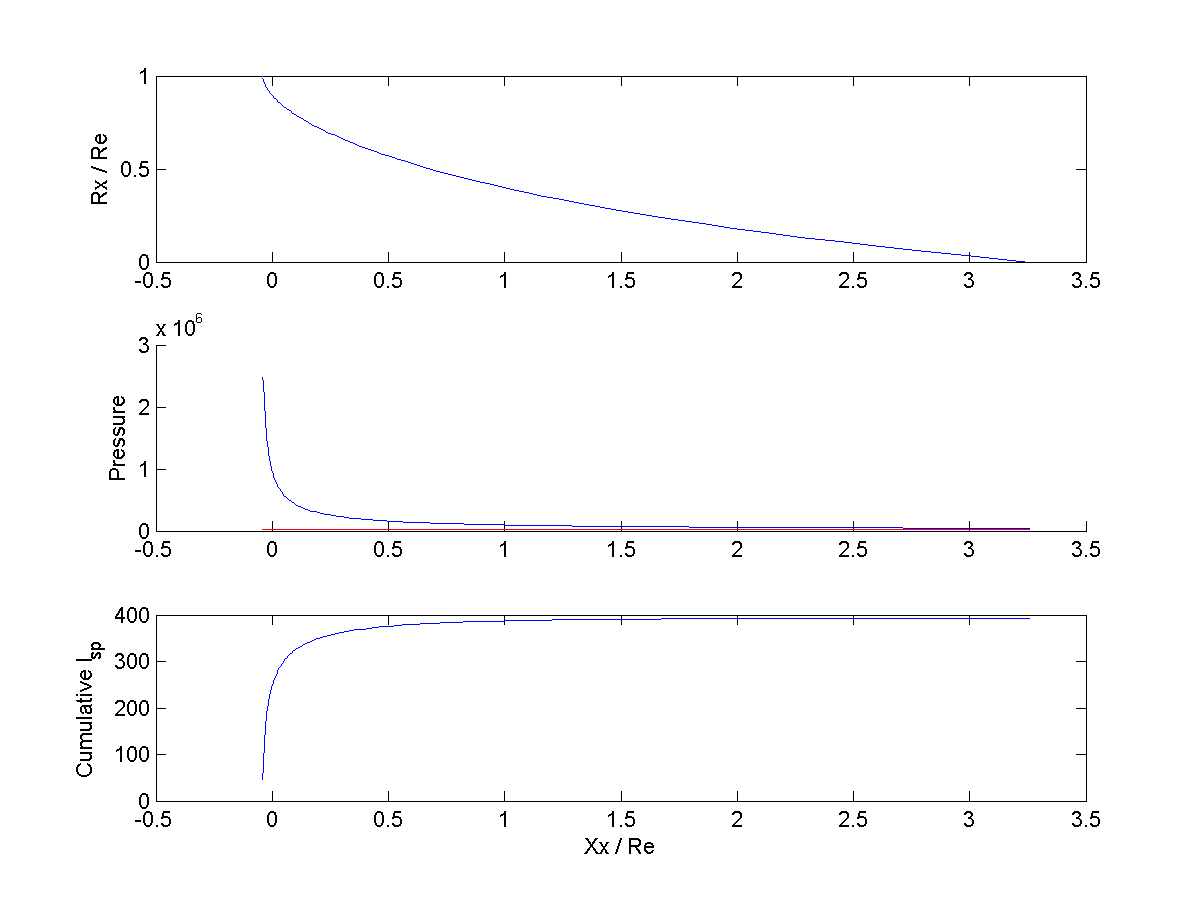
\includegraphics[width = 0.8\textwidth]{spike_contour.png}
\caption{Plots of spike radius (top), pressure (middle) and cumulative specific impulse (bottom) against spike length. Lengths are normalized by the nozzle radius.} 
\label{spike_contour}
\end{figure}

\section{Combustion Chamber}
The combustion chamber is to be made from graphite (for surfaces which will be in contact with combustion gasses) and steel (for the pressure vessel). A cavity of pressurized fuel gas insulates steel pressure vessel from heat of combustion chamber. As the pressure in this cavity is near the pressure in the combustion chamber, mechanical stress on the high-temperature graphite combustion chamber liner is minimized (Fig \ref{flow_concept} note 1). Injection orifices are positioned around the graphite combustion chamber liner so that fuel and oxidizer jets impinge, mixing the fluids for combustion (Fig \ref{flow_concept} note 2).
\begin{figure}[h!]
\centering
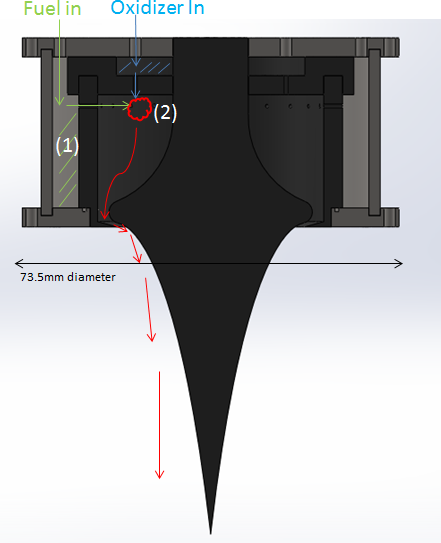
\includegraphics[width = 0.8\textwidth]{flow_concept.png}
\caption{A cross section of the combustion chamber and nozzle, annotated to show the flow of fuel and oxidizer} 
\label{flow_concept}
\end{figure}
The thermal and mechanical FEA simulation tools in Solidworks have been used to estimate the thermal and mechanical loads placed on the engine material by the combustion chamber pressure and temperature.\\
With a combustion chamber pressure of $\SI{5.0}{\mega\pascal}$ the simulation predicts a maximum stress of $\SI{92}{\mega\pascal}$ in the steel components (Fig \ref{engine_pressure}). 316 stainless steel's yield strength is $\SI{241}{\mega\pascal}$ at room temperature and $\SI{110}{\mega\pascal}$ at $\SI{1144}{\kelvin}$ \cite{316}.
\begin{figure}[h!]
\centering
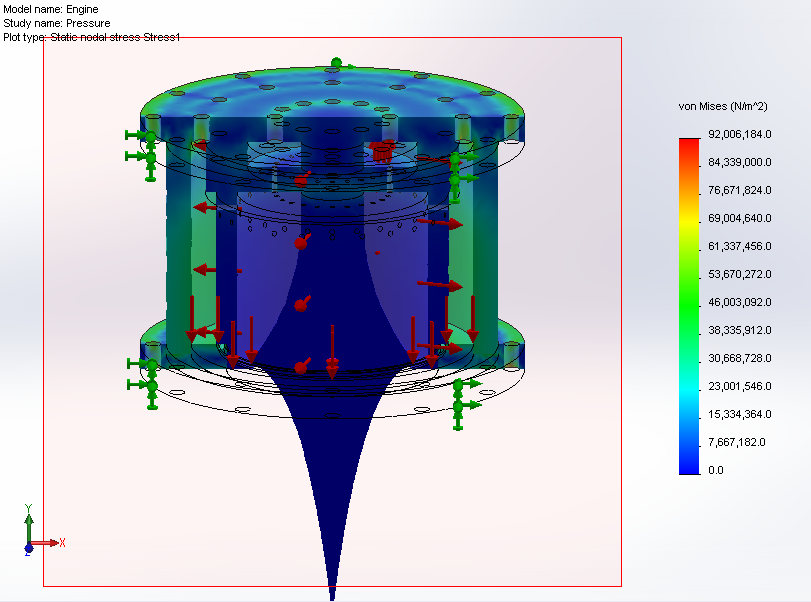
\includegraphics[width = 0.8\textwidth]{engine_pressure.png}
\caption{Stress in the engine structure due to $\SI{5.0}{\mega\pascal}$ chamber pressure} 
\label{engine_pressure}
\end{figure}
This thermal model shows that the fuel gas cavity successfully insulates the outer steel wall, keeping it below the maximum allowable temperature of $\SI{1144}{\kelvin}$. However the upper steel plate is excessively heated, indicating that a larger oxidizer cavity is required at the top of the engine (Fig \ref{engine_temperature}).
\begin{figure}[h!]
\centering
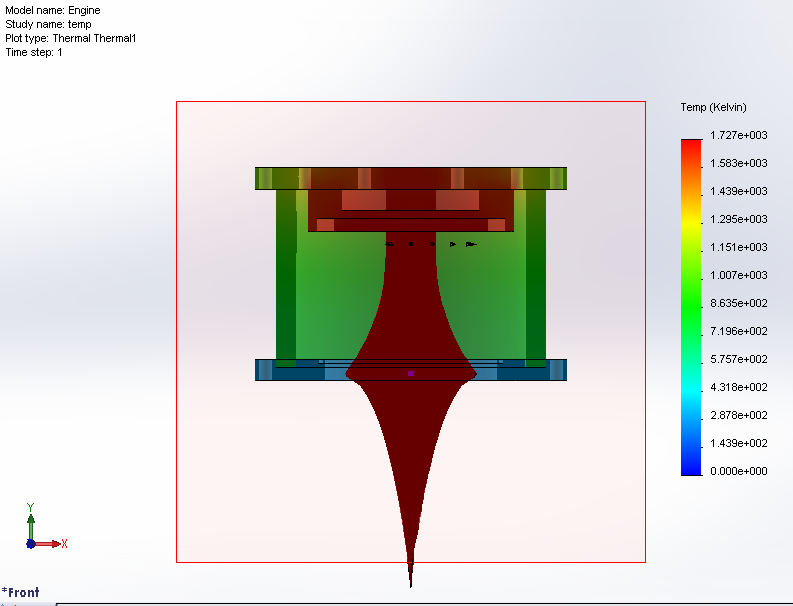
\includegraphics[width = 0.8\textwidth]{engine_temp_fail.png}
\caption{Temperature in the engine structure due to $\SI{1727}{\kelvin}$ combustion} 
\label{engine_temperature}
\end{figure}
\begin{thebibliography}{9}
	\bibitem{CEARUN} CEARUN. \emph{NASA.} http://cearun.grc.nasa.gov/.
	\bibitem{CCLee} C.C Lee. FORTRAN Programs for Plug Nozzle Design. \emph{NASA Marshal Space Flight Center.} 1963. http://ia700303.us.archive.org/24/items/nasa\_techdoc\_19630012259/19630012259.pdf.
	\bibitem{316} 316 Stainless Steel. \emph{AK Steel.} http://www.aksteel.com/pdf/markets\_products/stainless/austenitic/316\_316L\_Data\_Bulletin.pdf.
\end{thebibliography}
\end{document}
